\captionsetup{justification=centering,margin=0cm}
\label{cap:atividade2}  % Forma de referenciar o capítulo no comando \ref

%inicio do capitulo
\chapter[Atividade 2: AVALIANDO A “COMPLEXIDADE” DO CONTEÚDO DE UMA IMAGEM]{Atividade 2: AVALIANDO A “COMPLEXIDADE” DO CONTEÚDO DE UMA IMAGEM}

Após a compreensão das diferenças existentes entre os tipos de imagens, é hora de avaliar a complexidade de arquivos de imagem. Assim como foi feito no trabalho anterior, relacionado a áudio, iremos analisar um total de 50 imagens e definir a sua complexidade.

\hspace{1.5 cm} Antes de prosseguirmos, é válido ressaltar algumas informações importantes. Foram avaliadas no total 50 imagens no formato bmp, todas com resolução de 1200$\times$1200 e exatos 4.320.056 bytes. O parâmetro utilizado para medir a complexidade é o \textit{ratio}, isto é, o razão do tamanho após a compressão pelo tamanho original da imagem.

\hspace{1.5 cm} Com isto em mente, avaliamos imagem por imagem e tentamos prever o quão bem comprimido elas seriam. Descrever imagem por imagem seria bastante cansativo, assim segue a Tabela \ref{tab:classificacao_complexidade_imagens} para indicar em qual categoria cada imagem foi classificada e, logo após, um detalhamento geral de como foi feita a interpretação da compressão (caso seja necessário, algumas imagens específicas serão abordadas.)

\begin{table}[htbp]
\centering

\caption{Classificação da Complexidade das Imagens por Base Empírica.}
\label{tab:classificacao_complexidade_imagens}

\begin{tabularx}{\textwidth}{X|C|C|C}
    \hline
        
        \textbf{Baixa} & \textbf{Média Baixa} & Mé\textbf{dia Alta} & \textbf{Alta} \\ \hline
        IMG03, IMG05, IMG12, IMG15, IMG24, IMG29, IMG36, IMG46, IMG49 & IMG01, IMG06, IMG09, IMG16, IMG19, IMG26, IMG28, IMG31, IMG32, IMG41, IMG42, IMG45, IMG48 & IMG04, IMG07, IMG13, IMG17, IMG18, IMG21, IMG23, IMG25, IMG30, IMG34, IMG35, IMG37, IMG40, IMG44, IMG47, IMG50 & IMG02, IMG08, IMG10, IMG11, IMG14, IMG20, IMG22, IMG27, IMG33, IMG38, IMG39, IMG43 \\

    \hline
    
\end{tabularx}

\autoriaPropria

\end{table}

\hspace{1.5 cm} Para justificar as imagens de classificação baixa verificamos essencialmente duas variância de cores nos \textit{pixels} em vasta quantidade. Para melhor exemplificar nossa proposta, observe a Imagem \ref{fig:imagem_3}. Nela, há uma demarcação em vermelho, todo aquela campo possui uma variância muito pequena de \textit{pixels} em vasta quantidade na imagem, influenciando consideravelmente na nossa classificação. Acreditamos ser válida uma ressalva: essa percepção nem sempre é válida; levamos ela muito em consideração e, como diria o Pica-Pau, fomos "tapeados" por algumas imagens, como é o caso da "IMG05" e da "IMG24".

\begin{figure}[H]
    \centering
    
    \caption{Imagem 3 Adaptada}
    \label{fig:imagem_3}
    
    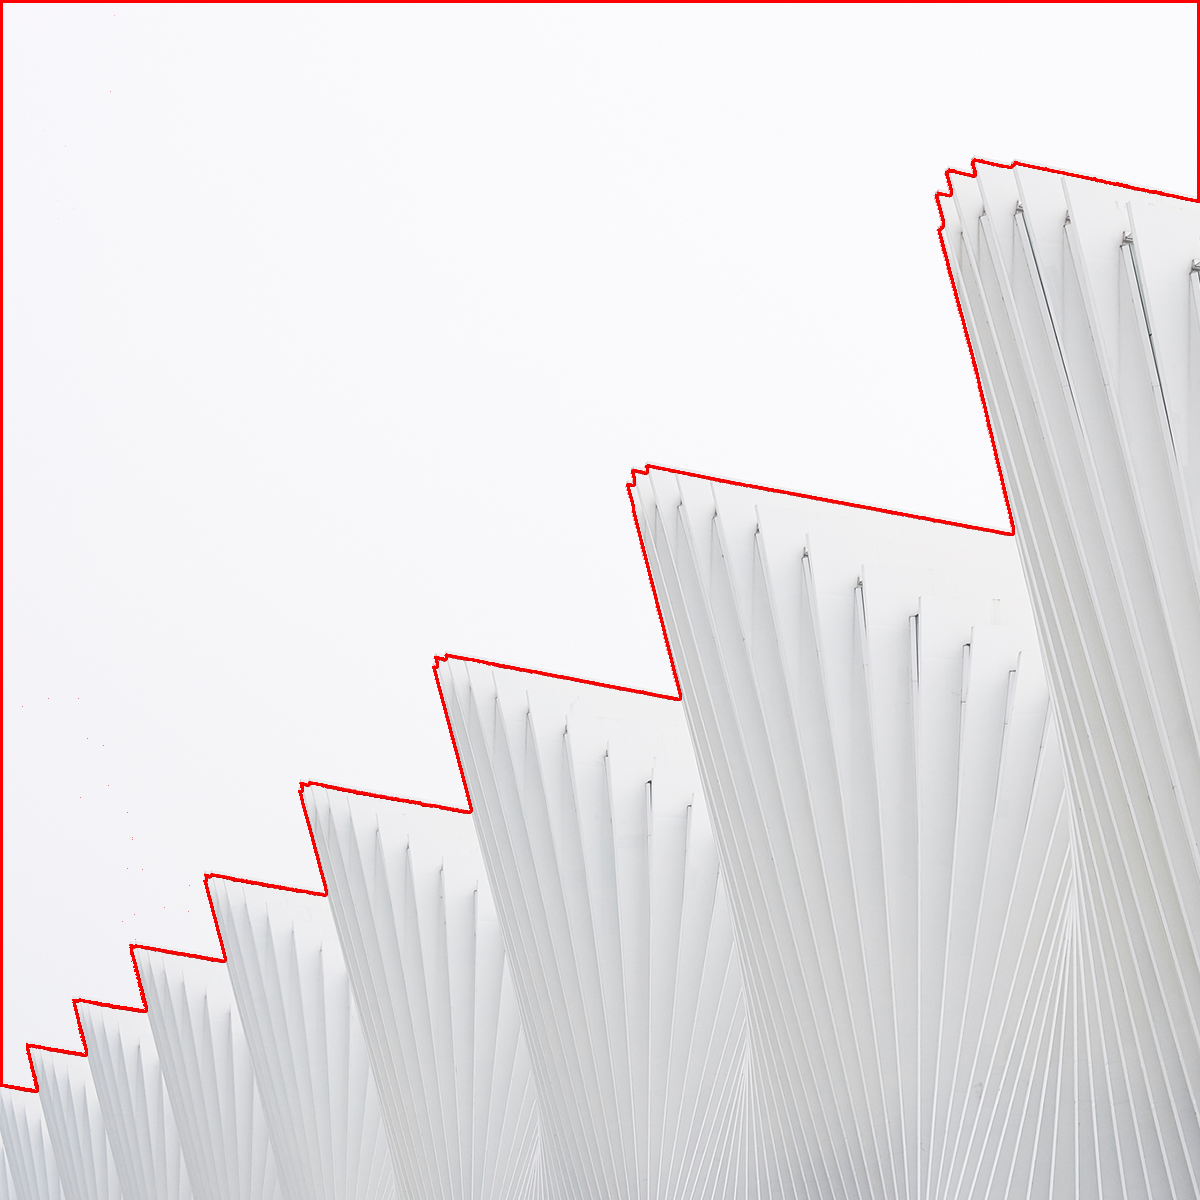
\includegraphics[scale=0.2]{Documeto/1-ElementosTextuais/1-Desenvolvimento/imagens-atividade2/IMG03.png}

    \fonteElementoGrafico{Adaptada das Imagens Fornecidas pelo Professor}
\end{figure}

\hspace{1.5 cm} As imagens de classificação média baixa e média alta são uma incógnita. Foi difícil definir quais valores práticos eram utilizados para definir a complexidade, ao ponto que muitas delas foram confundidas. No entanto, tentamos identificar a complexidade da imagem dividindo elas em alguns blocos. Acreditamos que tudo ficará mais claro se observar a Imagem \ref{fig:imagem_9}. Perceba que a imagem original foi recortada em 3 partes distintas. Acreditamos que o céu, que ocupa pouco mais de 45\% da imagem original, será bem comprimido, reduzindo consideravelmente seu tamanho. A parte da água tem uma quantidade considerável de detalhes, principalmente por causa dos reflexos, tornando ela não tão bem comprimível. Por fim, a parte central possui pontos de compressão, uma vez que elas são em suma brancas e possuem uma texturização não tão intensa em alguns pontos. Assim, conclui-se que ela aproxima-se de uma compressão baixa.

\begin{figure}[H]
    \centering
    
    \caption{Imagem 9 Adaptada}
    \label{fig:imagem_9}
    
    
\includegraphics[scale=0.25]{Documeto/1-ElementosTextuais/1-Desenvolvimento/imagens-atividade2/IMG09-corte.png}

    \fonteElementoGrafico{Adaptada das Imagens Fornecidas pelo Professor}
\end{figure}

\hspace{1.5 cm} Por fim, para classificar uma imagem com categoria alta, utilizou-se o mesmo método anterior, mas com um toque a mais de preguiça. Sempre que uma imagem que cansava muito os olhos ou possuía tanta coisa ao ponto de nem termos ideia de como classificá-lá em um primeiro momento, já tínhamos um indício de que ela seria pouco comprimida. Depois, uma análise um pouco menos empírica era feita para averiguar se era uma sensação que fazia sentido e então era feita a classificação.